% *** Authors should verify (and, if needed, correct) their LaTeX system  ***
% *** with the testflow diagnostic prior to trusting their LaTeX platform ***
% *** with production work. IEEE's font choices can trigger bugs that do  ***
% *** not appear when using other class files.                            ***
% The testflow support page is at:
% http://www.michaelshell.org/tex/testflow/


%%*************************************************************************
%% Legal Notice:
%% This code is offered as-is without any warranty either expressed or
%% implied; without even the implied warranty of MERCHANTABILITY or
%% FITNESS FOR A PARTICULAR PURPOSE!
%% User assumes all risk.
%% In no event shall IEEE or any contributor to this code be liable for
%% any damages or losses, including, but not limited to, incidental,
%% consequential, or any other damages, resulting from the use or misuse
%% of any information contained here.
%%
%% All comments are the opinions of their respective authors and are not
%% necessarily endorsed by the IEEE.
%%
%% This work is distributed under the LaTeX Project Public License (LPPL)
%% ( http://www.latex-project.org/ ) version 1.3, and may be freely used,
%% distributed and modified. A copy of the LPPL, version 1.3, is included
%% in the base LaTeX documentation of all distributions of LaTeX released
%% 2003/12/01 or later.
%% Retain all contribution notices and credits.
%% ** Modified files should be clearly indicated as such, including  **
%% ** renaming them and changing author support contact information. **
%%
%% File list of work: IEEEtran.cls, New_IEEEtran_how-to.pdf, bare_jrnl_new_sample4.tex,
%%*************************************************************************
\PassOptionsToPackage{unicode}{hyperref}
\PassOptionsToPackage{hyphens}{url}
\PassOptionsToPackage{dvipsnames,svgnames,x11names}{xcolor}
% Note that the a4paper option is mainly intended so that authors in
% countries using A4 can easily print to A4 and see how their papers will
% look in print - the typesetting of the document will not typically be
% affected with changes in paper size (but the bottom and side margins will).
% Use the testflow package mentioned above to verify correct handling of
% both paper sizes by the user's LaTeX system.
%
% Also note that the "draftcls" or "draftclsnofoot", not "draft", option
% should be used if it is desired that the figures are to be displayed in
% draft mode.
%
\documentclass[
  journal,
]{IEEEtran}%
% If IEEEtran.cls has not been installed into the LaTeX system files,
% manually specify the path to it like:
% \documentclass[journal]{../sty/IEEEtran}
\usepackage[cmex10]{amsmath}
\usepackage{amssymb}
\usepackage{iftex}
\ifPDFTeX
  \usepackage[T1]{fontenc}
  \usepackage[utf8]{inputenc}
  \usepackage{textcomp} % provide euro and other symbols
\else % if luatex or xetex
  \usepackage{unicode-math} % this also loads fontspec
  \defaultfontfeatures{Scale=MatchLowercase}
  \defaultfontfeatures[\rmfamily]{Ligatures=TeX,Scale=1}
\fi
%\usepackage{lmodern}
\ifPDFTeX\else
\fi
% Use upquote if available, for straight quotes in verbatim environments
\IfFileExists{upquote.sty}{\usepackage{upquote}}{}
\IfFileExists{microtype.sty}{% use microtype if available
  \usepackage[]{microtype}
  \UseMicrotypeSet[protrusion]{basicmath} % disable protrusion for tt fonts
}{}
\makeatletter
\parindent    1.0em
\ifCLASSOPTIONcompsoc
  \parindent    1.5em
\fi
\makeatother
\usepackage{xcolor}
\setlength{\emergencystretch}{3em} % prevent overfull lines

\setcounter{secnumdepth}{5}
% Make \paragraph and \subparagraph free-standing
\ifx\paragraph\undefined\else
  \let\oldparagraph\paragraph
  \renewcommand{\paragraph}[1]{\oldparagraph{#1}\mbox{}}
\fi
\ifx\subparagraph\undefined\else
  \let\oldsubparagraph\subparagraph
  \renewcommand{\subparagraph}[1]{\oldsubparagraph{#1}\mbox{}}
\fi


\providecommand{\tightlist}{%
  \setlength{\itemsep}{0pt}\setlength{\parskip}{0pt}}\usepackage{longtable,booktabs,array}
\usepackage{calc} % for calculating minipage widths
% Correct order of tables after \paragraph or \subparagraph
\usepackage{etoolbox}
\makeatletter
\patchcmd\longtable{\par}{\if@noskipsec\mbox{}\fi\par}{}{}
\makeatother
% Allow footnotes in longtable head/foot
\IfFileExists{footnotehyper.sty}{\usepackage{footnotehyper}}{\usepackage{footnote}}
\makesavenoteenv{longtable}
\usepackage{graphicx}
\makeatletter
\def\maxwidth{\ifdim\Gin@nat@width>\linewidth\linewidth\else\Gin@nat@width\fi}
\def\maxheight{\ifdim\Gin@nat@height>\textheight\textheight\else\Gin@nat@height\fi}
\makeatother
% Scale images if necessary, so that they will not overflow the page
% margins by default, and it is still possible to overwrite the defaults
% using explicit options in \includegraphics[width, height, ...]{}
\setkeys{Gin}{width=\maxwidth,height=\maxheight,keepaspectratio}
% Set default figure placement to htbp
\makeatletter
\def\fps@figure{htbp}
\makeatother
\newlength{\cslhangindent}
\setlength{\cslhangindent}{1.5em}
\newlength{\csllabelwidth}
\setlength{\csllabelwidth}{3em}
\newlength{\cslentryspacingunit} % times entry-spacing
\setlength{\cslentryspacingunit}{\parskip}
\newenvironment{CSLReferences}[2] % #1 hanging-ident, #2 entry spacing
 {% don't indent paragraphs
  \setlength{\parindent}{0pt}
  % turn on hanging indent if param 1 is 1
  \ifodd #1
  \let\oldpar\par
  \def\par{\hangindent=\cslhangindent\oldpar}
  \fi
  % set entry spacing
  \setlength{\parskip}{#2\cslentryspacingunit}
 }%
 {}
\usepackage{calc}
\newcommand{\CSLBlock}[1]{#1\hfill\break}
\newcommand{\CSLLeftMargin}[1]{\parbox[t]{\csllabelwidth}{#1}}
\newcommand{\CSLRightInline}[1]{\parbox[t]{\linewidth - \csllabelwidth}{#1}\break}
\newcommand{\CSLIndent}[1]{\hspace{\cslhangindent}#1}

\usepackage{physics}
\usepackage[version=3]{mhchem}
\usepackage{orcidlink}
\usepackage{float}
\floatplacement{table}{htb}
\makeatletter
\makeatother
\makeatletter
\makeatother
\makeatletter
\@ifpackageloaded{caption}{}{\usepackage{caption}}
\AtBeginDocument{%
\ifdefined\contentsname
  \renewcommand*\contentsname{Table of contents}
\else
  \newcommand\contentsname{Table of contents}
\fi
\ifdefined\listfigurename
  \renewcommand*\listfigurename{List of Figures}
\else
  \newcommand\listfigurename{List of Figures}
\fi
\ifdefined\listtablename
  \renewcommand*\listtablename{List of Tables}
\else
  \newcommand\listtablename{List of Tables}
\fi
\ifdefined\figurename
  \renewcommand*\figurename{Fig.}
\else
  \newcommand\figurename{Fig.}
\fi
\ifdefined\tablename
  \renewcommand*\tablename{Table}
\else
  \newcommand\tablename{Table}
\fi
}
\@ifpackageloaded{float}{}{\usepackage{float}}
\floatstyle{ruled}
\@ifundefined{c@chapter}{\newfloat{codelisting}{h}{lop}}{\newfloat{codelisting}{h}{lop}[chapter]}
\floatname{codelisting}{Listing}
\newcommand*\listoflistings{\listof{codelisting}{List of Listings}}
\usepackage{amsthm}
\theoremstyle{plain}
\newtheorem{theorem}{Theorem}[section]
\theoremstyle{remark}
\AtBeginDocument{\renewcommand*{\proofname}{Proof}}
\newtheorem*{remark}{Remark}
\newtheorem*{solution}{Solution}
\makeatother
\makeatletter
\@ifpackageloaded{caption}{}{\usepackage{caption}}
\@ifpackageloaded{subcaption}{}{\usepackage{subcaption}}
\makeatother
\makeatletter
\@ifpackageloaded{tcolorbox}{}{\usepackage[skins,breakable]{tcolorbox}}
\makeatother
\makeatletter
\@ifundefined{shadecolor}{\definecolor{shadecolor}{rgb}{.97, .97, .97}}
\makeatother
\makeatletter
\makeatother
\makeatletter
\makeatother
\usepackage[skip=2pt,font=footnotesize]{caption}
%\captionsetup{format=myformat}
\makeatletter
%\setlength{\cslhangindent}{0pt plus .5pt}
\providecommand{\bibfont}{\footnotesize}
\let\CSLReferences@rig=\CSLReferences
\renewcommand{\CSLReferences}[2]{
\bibfont\settowidth\csllabelwidth{[999]}
\CSLReferences@rig{#1}{#2}
\vskip 0.3\baselineskip plus 0.1\baselineskip minus 0.1\baselineskip%
}
\makeatother
\ifLuaTeX
  \usepackage{selnolig}  % disable illegal ligatures
\fi
\IfFileExists{bookmark.sty}{\usepackage{bookmark}}{\usepackage{hyperref}}
\IfFileExists{xurl.sty}{\usepackage{xurl}}{} % add URL line breaks if available
\urlstyle{same} % disable monospaced font for URLs
\hypersetup{
  pdftitle={A Sample Article Using quarto-ieee for IEEE Journal and Transactions},
  pdfauthor={David Folio; John Doe},
  pdfkeywords={IEEE, IEEEtran, journal, Quarto, Pandoc, template},
  colorlinks=true,
  linkcolor={blue},
  filecolor={Maroon},
  citecolor={Blue},
  urlcolor={Blue},
  pdfcreator={LaTeX via pandoc}}

% *** Do not adjust lengths that control margins, column widths, etc. ***
% *** Do not use packages that alter fonts (such as pslatex).         ***
% There should be no need to do such things with IEEEtran.cls V1.6 and later.
% (Unless specifically asked to do so by the journal or conference you plan
% to submit to, of course. )


% correct bad hyphenation here
\hyphenation{op-tical net-works semi-conduc-tor}

%
% paper title
% can use linebreaks \\ within to get better formatting as desired
% Do not put math or special symbols in the title.
% paper title
% can use linebreaks \\ within to get better formatting as desired
% Do not put math or special symbols in the title.
\title{A Sample Article Using \texttt{quarto-ieee} for IEEE Journal and
Transactions}

\author{
\thanks{The \texttt{quarto-ieee} template is freely available under the
MIT license on github: \url{https://github.com/dfolio/quarto-ieee}.}
David Folio\orcidlink{0000-0001-9430-6091},~\IEEEmembership{Member,
IEEE}
and~John Doe%
\thanks{David Folio is with Laboratoire Prisme, INSA Centre Val de
Loire, Bourges, 18800 France%
  Corresponding author: david.folio@insa-cvl.fr
}
\thanks{Unknown affiliation}
%by-author.affiliations
\thanks{John Doe is with Anonymous University%
}
%by-author.affiliations
\thanks{Template created June 23, 2023; revised February 27, 2024.}
}
\begin{document}

% The paper headers
\markboth{Journal XXX, Month Year}{D. Folio: A Sample Article Using
quarto-ieee}

% use for special paper notices

% make the title area
\maketitle

% As a general rule, do not put math, special symbols or citations
% in the abstract or keywords.
\begin{abstract}
This document describes the most common article elements and how to use
the \texttt{quarto-ieee} class with Pandoc/Quarto-Markdown to produce
files that are suitable for submission to IEEE journals.
\texttt{quarto-ieee} can produce conference, journal, and technical note
(correspondence) papers with a suitable choice of class options. It
intends to generate PDF and HTML outputs that closely mimick what IEEE
would generate.
\end{abstract}
% Note that keywords are not normally used for peerreview papers.
\begin{IEEEkeywords}
IEEE, IEEEtran, journal, Quarto, Pandoc, template
\end{IEEEkeywords}

% For peer review papers, you can put extra information on the cover
% page as needed:
% \ifCLASSOPTIONpeerreview
% \begin{center} \bfseries EDICS Category: 3-BBND \end{center}
% \fi
%
% For peerreview papers, this IEEEtran command inserts a page break and
% creates the second title. It will be ignored for other modes.
% \IEEEpeerreviewmaketitle

\ifdefined\Shaded\renewenvironment{Shaded}{\begin{tcolorbox}[borderline west={3pt}{0pt}{shadecolor}, boxrule=0pt, frame hidden, enhanced, interior hidden, sharp corners, breakable]}{\end{tcolorbox}}\fi

\hypertarget{sec-intro}{%
\section{Introduction}\label{sec-intro}}

\IEEEPARstart{T}{his} file is intended to serve as a ``sample article
file'' for IEEE journal papers produced with (Pandoc/Quarto)-Markdown
using \texttt{IEEEtran.cls} version 1.8b and later for the PDF output.
It is based on \texttt{bare\_jrnl\_new\_sample4.tex} provided by IEEE
Publication Technology, Staff and available from
\url{https://template-selector.ieee.org/}. The most common elements are
covered in the simplified and updated instructions in
\texttt{New\_IEEEtran\_how-to.pdf}. For less common elements you can
refer back to the original \texttt{IEEEtran\_HOWTO.pdf}. It is assumed
that the reader has a basic working knowledge of {\LaTeX}
\protect\hyperlink{ref-mittelbach2023latex}{{[}1{]}} and of
(Pandoc/Quarto)-Markdown
\protect\hyperlink{ref-MacFarlane_Pandoc}{{[}2{]}},
\protect\hyperlink{ref-Allaire_Quarto_2022}{{[}3{]}} markup.

\hypertarget{the-design-intent-and-limitations-of-this-templates}{%
\section{The Design, Intent, and Limitations of this
Templates}\label{the-design-intent-and-limitations-of-this-templates}}

The \texttt{quarto-ieee} template is intended to \textbf{approximate the
final look and page length of the articles/papers} either in PDF output
or HTML output. \textbf{They are NOT intended to be the final produced
work that is displayed in print or on IEEEXplore\textsuperscript{®}}.
They will help to give the authors an approximation of the number of
pages and layout that will be in the final version.

\hypertarget{unsuported-feature-and-limitations}{%
\subsection{Unsuported feature and
limitations}\label{unsuported-feature-and-limitations}}

Although most of the {\LaTeX} and \texttt{IEEEtran.cls} commands and
environment are supported, there are some limitations when trying to
export to a format other than PDF (e.g.~HTML output). For PDF output,
the reader can use the {\LaTeX} command directly. However, this may
break other output formats.\\
It can be can reported the following limitations of the
\texttt{quarto-ieee} template: - Several authors with same affiliation
produce weird output. In such case, it is recommended to use
\texttt{note} and \texttt{tex-author-no-affiliation:\ true}. - For
\texttt{PDF} output - \texttt{quarto-ieee} use a hack to handle the
\texttt{longtable} issue with 2-column {\LaTeX} documents\footnote{{[}``\emph{\href{https://github.com/jgm/pandoc/issues/1023\%3E}{longtable
  not compatible with 2-column LaTeX documents}}'',}. But, in some
cases, a page overflow may occur (see also Section~\ref{sec-tables}). -
For \texttt{HTML} output - The default Quarto toc is used, so the table
of contents (toc) display is not the same as on
\href{https://ieeexplore.ieee.org/}{IEEEXplore®}. - Footnote are put at
the end of document, while on
\href{https://ieeexplore.ieee.org/}{IEEEXplore®} there are placed in the
accordion. - Figures are not placed in the accordion. -
\href{https://ieeexplore.ieee.org/}{IEEEXplore®} specifics
(e.g.~citation metrics, etc.) - The \texttt{HTML} output is a Quarto
citeable article \protect\hyperlink{ref-quarto-citation}{{[}4{]}}, so a
citation appendix is automatically added to the article end.

\hypertarget{contributing}{%
\subsection{Contributing}\label{contributing}}

If you want to improve the \texttt{quarto-ieee} template or need some
specific features do not hesitate to submit Pull Request\footnote{Go to
  the PR page: \url{https://github.com/dfolio/quarto-ieee/pulls}} (it is
considered good practice to open an issue for discussion before working
on a pull request for a new feature).

\hypertarget{some-random-text}{%
\section{Some random text}\label{some-random-text}}

For some of the remainder of this sample we will use dummy text to fill
out paragraphs rather than use live text that may violate a copyright.
\IEEEpubidadjcol\\
Lorem ipsum dolor sit amet, consectetur adipiscing elit. Duis cursus
nisl eget tempor porta. Proin dapibus dictum quam a commodo. Mauris
congue scelerisque eros a porta. Proin blandit nulla sapien, et pretium
justo dictum non. Vivamus ultricies, elit eu posuere placerat, sapien
est condimentum nisl, at tincidunt tortor dolor ac ligula. Suspendisse
pulvinar libero quis eros finibus sodales. Vivamus mattis est eget
imperdiet luctus. Morbi eget posuere metus. Nam egestas elit lectus, eu
tincidunt odio viverra sed. Sed sit amet metus rutrum, ultricies elit
in, finibus felis. Integer lobortis dui ante, eget placerat lorem
laoreet eu.

Nullam mi ligula, luctus a orci ut, tincidunt varius augue. Vestibulum
ante ipsum primis in faucibus orci luctus et ultrices posuere cubilia
curae; Donec sed sem risus. Nam eleifend ultrices elit, vitae posuere
tellus interdum et. Nam id nisl at elit malesuada malesuada. Suspendisse
viverra ipsum libero, vel pharetra sem maximus sed. Nunc vel est
fringilla, rutrum diam eu, egestas quam. Vivamus lobortis blandit velit,
commodo finibus mauris. Quisque vel lacus ipsum. Pellentesque quis nulla
ipsum.

Aenean in hendrerit quam. Orci varius natoque penatibus et magnis dis
parturient montes, nascetur ridiculus mus. Aliquam tincidunt vehicula
dignissim. In quis aliquet lectus, ac vestibulum elit. Quisque a magna
viverra quam viverra faucibus. Nulla ornare tortor at mollis viverra.
Curabitur vel porta dui. Etiam ipsum elit, egestas eget lacus nec,
laoreet iaculis lacus. In iaculis risus ac tincidunt viverra. Maecenas
tempor iaculis odio quis aliquet.\\
Maecenas ac posuere turpis. Fusce est dui, dapibus sed odio eget,
eleifend facilisis felis. Nam gravida varius enim, ornare tincidunt urna
ullamcorper ut. Donec sit amet eros ac lacus placerat rutrum ut non
dolor. Nulla tincidunt nunc massa, sed euismod dui feugiat vitae.
Integer tempus risus rutrum tellus interdum, eu aliquet sapien rutrum.
Nunc feugiat varius lacus sed laoreet. Integer euismod tellus nisi, id
scelerisque sem sagittis eu. Suspendisse at orci vel neque varius tempor
nec vitae odio. Integer elementum elementum fermentum. Morbi in turpis
cursus, lacinia arcu et, semper orci.

\hypertarget{front-matter}{%
\section{Front matter}\label{front-matter}}

Most Quarto's authors and affiliations schemes
\protect\hyperlink{ref-quarto-funding}{{[}5{]}} are supported in the
YAML front matter to render authors as requested by IEEE journals in PDF
and HTML outputs. When provided to an author, the \texttt{note} entry is
rendered as a \texttt{\textbackslash{}thanks\{\}} in \texttt{PDF} output
(ignored in \texttt{HTML} output). Additionally, the reader may add to
an author a \texttt{photo:\ path/to/photograph.png} with a \texttt{bio}
metadata entries to generate a \texttt{IEEEbiography}, while a sole
\texttt{bio} generates a \texttt{IEEEbiographynophoto} (these features
is used both in \texttt{PDF} and \texttt{HTML} outputs).\\
The \texttt{funding} entry is also used in both PDF and HTML outputs
\protect\hyperlink{ref-quarto-funding}{{[}5{]}}. At version v1.1.1, only
the \texttt{funding.statement} is used. Similarly, \texttt{citation}
entry is supported to make the HTML output a ``\emph{citeable
article}''~\protect\hyperlink{ref-quarto-citation}{{[}4{]}}.

\hypertarget{some-common-elements}{%
\section{Some Common Elements}\label{some-common-elements}}

\hypertarget{sections-and-subsections}{%
\subsection{Sections and Subsections}\label{sections-and-subsections}}

As stated in the \texttt{IEEEtran} template enumeration of section
headings is desirable, but not required. When numbered, it should be
consistent throughout the article, that is, all headings and all levels
of section headings in the article should be enumerated. Primary
headings are designated with Roman numerals, secondary with capital
letters, tertiary with Arabic numbers; and quaternary with lowercase
letters. References and Acknowledgment headings are unlike all other
section headings in text. They are never enumerated. They are simply
primary headings without labels, regardless of whether the other
headings in the article are enumerated.

The following Section~\ref{sec-Markdown} shows some basic usage and
capabilities of \texttt{quarto-ieee}.

\hypertarget{sec-Markdown}{%
\subsection{Markdown basics}\label{sec-Markdown}}

The reader can easily find many documentations on how to write using the
(Pandoc/Quarto) Markdown syntax. The \texttt{quarto-ieee} template
relies mainly on the Markdown markup supported by Quarto
\protect\hyperlink{ref-quarto-markdown}{{[}6{]}}, which is build based
on Pandoc \protect\hyperlink{ref-MacFarlane_Pandoc}{{[}2{]}},
\protect\hyperlink{ref-Allaire_Quarto_2022}{{[}3{]}}. Below are some
basic examples of usage of the Markdown markup (to save space, it is
better to consult the original Quarto document \texttt{template.qmd}).

\hypertarget{display-equations}{%
\subsubsection{Display equations}\label{display-equations}}

To write equations use \texttt{\$} delimiters for inline formula or
\texttt{\$\$} for block one. To number the equations, it is recommended
to use classic equation environments provided by {\LaTeX} and to use
\texttt{\textbackslash{}eqref\{\}} (or \texttt{\textbackslash{}ref\{\}})
for cross-referencing. For example: \begin{equation}\label{eq:1}
{{\chi}_a}=\text{diag}\left(\frac{{\chi}}{1+n_a{\chi}},\frac{{\chi}}{1+n_b{\chi}},\frac{{\chi}}{1+n_b{\chi}}\right),
\end{equation} \begin{align}
a & = b + c \label{eq:2} \\
c & = d + e \label{eq:3}
\end{align}

\begin{equation}\label{eq:4}
\begin{cases}
    1&=n_a+2n_b \\
    n_a&=\dfrac{1-{\varepsilon}^2}{2{\varepsilon}^3}\left(\log\left(\dfrac{1+{\varepsilon}}{1-{\varepsilon}}\right)-2{\varepsilon}\right)
\end{cases}
\end{equation} The above equation is cross-referenced as \eqref{eq:1},
\eqref{eq:2}, \eqref{eq:3} and \eqref{eq:4}.

For now, avoid using the Quarto cross-references that use of
\texttt{\$\$\ \$\$} with \texttt{\#eq-} label. It works properly only
for PDF output, but there are some issues with HTML\footnote{See the
  issue here \url{https://github.com/quarto-dev/quarto-cli/issues/2275}}
output.

\begin{remark}

\texttt{quarto-ieee} template also supports the
\href{https://ctan.org/pkg/mhchem}{\texttt{mhchem}} (for chemical
equation) and \href{https://ctan.org/pkg/physics}{\texttt{physics}} (for
flexible macros for typesetting equations) {\LaTeX} packages and
\href{https://docs.mathjax.org/en/latest/input/tex/extensions/index.html}{Mathjax
extensions}.

\end{remark}

\hypertarget{theorems-proofs-and-remarks}{%
\subsubsection{Theorems, Proofs and
Remarks}\label{theorems-proofs-and-remarks}}

To include a reference-able theorem, create a div with a \texttt{\#thm-}
label. A theorem name is specified via the first heading in the block.
For example:

\begin{theorem}[Line]\protect\hypertarget{thm-line}{}\label{thm-line}

The equation of any straight line, called a linear equation, can be
written as:

\[
y = mx + b
\]

\end{theorem}

The theorem is cross-referenced as Theorem~\ref{thm-line}.

There are a number of theorem variations supported by
\href{https://quarto.org/docs/authoring/cross-references.html\#theorems-and-proofs}{Quarto},
each with their own label prefix:

\begin{itemize}
\tightlist
\item
  \texttt{\#thm-} for Theorem;
\item
  \texttt{\#lem-} for Lemma;
\item
  \texttt{\#cor-} for Corollary
\item
  \texttt{\#prp-} for Proposition;
\item
  \texttt{\#cnj-} for Conjecture;
\item
  \texttt{\#def-} for Definition;
\item
  \texttt{\#exm-} for Example;
\item
  \texttt{\#exr-} for Exercise.
\end{itemize}

The \texttt{proof}, \texttt{remark} and \texttt{solution} environments
generally receive similar typesetting as theorems. However they are not
numbered (and therefore cannot be cross-referenced). To create these
environments just use them as the class name of a div such as:

\begin{solution}[The solution]

An example of solution environment.

\end{solution}

\hypertarget{figures}{%
\subsubsection{Figures}\label{figures}}

An image with nonempty alt text will be rendered as a figure with a
caption with Pandoc and Quarto. Quarto includes a different features to
simplify the use of figures and subfigures. Here, it is recommended to
use div block with \texttt{\#fig-} label to embed your Figures.

\begin{figure}

{\centering 

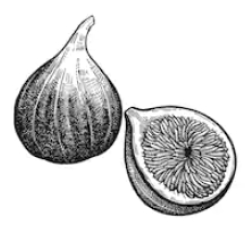
\includegraphics[width=0.3\textwidth,height=\textheight]{fig1.png}

}

\caption{\label{fig-1}An example of figure.}

\end{figure}

\begin{figure}

\begin{minipage}[t]{0.50\linewidth}

{\centering 

\raisebox{-\height}{

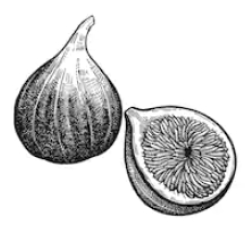
\includegraphics{fig1.png}

}

}

\subcaption{\label{fig-2a}}
\end{minipage}%
%
\begin{minipage}[t]{0.50\linewidth}

{\centering 

\raisebox{-\height}{

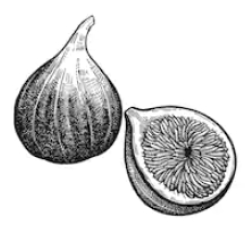
\includegraphics{fig1.png}

}

}

\subcaption{\label{fig-2b}}
\end{minipage}%

\caption{\label{fig-2}An example with sub-figure.}

\end{figure}

The figures is cross-referenced as Fig.~\ref{fig-2} and even the
sub-figures as Fig.~\ref{fig-2b}.

\hypertarget{sec-tables}{%
\subsubsection{Tables}\label{sec-tables}}

Similarly, many kind of tables may be used with Pandoc and Quarto. The
latter also includes different features to simplify the table output. To
make tables cross-referenceable use a label with a \texttt{\#tbl-}
prefix.\\
However, it is recommended to avoid using the commonly used single
Markdown table known as a `pipe table'. In fact, Pandoc Markdown uses
the {\LaTeX} \texttt{longtable} package, which does not support the
two-column mode, which is required for most \texttt{IEEEtran} journals.
\texttt{quarto-ieee} uses a hack to temporarily switch to one-column
mode. However, this hack may break the page layout. To overcome this
issue, a basic way is to use code cells (as for Table~\ref{tbl-other}).
Quarto is a multi-language and it uses \texttt{Knitr} to execute
\texttt{R} code and can execute Python code blocks within Markdown.

\begin{table}

\caption{\label{tbl-panel}Main
Caption}\begin{minipage}[t]{0.50\linewidth}
\subcaption{\label{tbl-first}First Table}

{\centering 

\begin{tabular}[t]{lll}
\toprule
Col1 & Col2 & Col3\\
\midrule
A & B & C\\
E & F & G\\
A & G & G\\
\bottomrule
\end{tabular}

}

\end{minipage}%
%
\begin{minipage}[t]{0.50\linewidth}
\subcaption{\label{tbl-second}Second Table}

{\centering 

\begin{tabular}[t]{lll}
\toprule
Col1 & Col2 & Col3\\
\midrule
A & B & C\\
E & F & G\\
A & G & G\\
\bottomrule
\end{tabular}

}

\end{minipage}%

\end{table}

The Tables are cross-referenced as Table~\ref{tbl-panel} for details,
especially Table~\ref{tbl-second}. There is also Table~\ref{tbl-other}.

\hypertarget{tbl-other}{}
\begin{table}
\caption{\label{tbl-other}A table }\tabularnewline

\centering
\begin{tabular}{lll}
\toprule
Col1 & Col2 & Col3\\
\midrule
A & D & G\\
B & E & H\\
C & F & I\\
\bottomrule
\end{tabular}
\end{table}

\hypertarget{bibliography}{%
\subsection{Bibliography}\label{bibliography}}

IEEE journal should normally use IEEEtran\footnote{IEEEtran BibTeX style
  support page is:
  \url{http://www.michaelshell.org/tex/ieeetran/bibtex/}}
\textsc{Bib}{\TeX} style. Nevertheless, Pandoc and Quarto do support
\textsc{Bib}{\TeX} with natbib or biblatex. However, neither is
officially recommended for normal IEEE use. For this reason,
\texttt{quarto-ieee} uses \texttt{citeproc} with the \texttt{ieee} CSL
style sheet.

\hypertarget{conclusions}{%
\section{Conclusions}\label{conclusions}}

The conclusion goes here.

\hypertarget{acknowledgment}{%
\section*{Acknowledgment}\label{acknowledgment}}
\addcontentsline{toc}{section}{Acknowledgment}

This should be a simple paragraph before the References to thank those
individuals and institutions who have supported your work on this
article.

\appendix[An Appendix]{}

Use \texttt{{[}{]}\{.appendix\ options="An\ Appendix"\}} markup if you
have a single appendix. \texttt{IEEEtran} state that to do not use
\texttt{\textbackslash{}section\{\}} anymore after
\texttt{\textbackslash{}appendix}.

\hypertarget{references}{%
\section*{References}\label{references}}
\addcontentsline{toc}{section}{References}

\hypertarget{refs}{}
\begin{CSLReferences}{0}{0}
\leavevmode\vadjust pre{\hypertarget{ref-mittelbach2023latex}{}}%
\CSLLeftMargin{{[}1{]} }%
\CSLRightInline{F. Mittelbach and U. Fischer, \emph{The {LaTeX}
companion}, 3rd ed. {Addison Wesley Professional}, 2023. }

\leavevmode\vadjust pre{\hypertarget{ref-MacFarlane_Pandoc}{}}%
\CSLLeftMargin{{[}2{]} }%
\CSLRightInline{J. MacFarlane, A. Krewinkel, and J. Rosenthal,
{``{Pandoc}.''} {[}Online{]}. Available:
\url{https://github.com/jgm/pandoc}}

\leavevmode\vadjust pre{\hypertarget{ref-Allaire_Quarto_2022}{}}%
\CSLLeftMargin{{[}3{]} }%
\CSLRightInline{J. J. Allaire, C. Teague, C. Scheidegger, Y. Xie, and C.
Dervieux, {``{Quarto}.''} Jan-2022 {[}Online{]}. Available:
\url{https://github.com/quarto-dev/quarto-cli}}

\leavevmode\vadjust pre{\hypertarget{ref-quarto-citation}{}}%
\CSLLeftMargin{{[}4{]} }%
\CSLRightInline{{``Quarto - {Creating Citeable Articles}.''}
{[}Online{]}. Available:
\url{https://quarto.org/docs/authoring/create-citeable-articles.html}.
{[}Accessed: 25-Oct-2023{]}}

\leavevmode\vadjust pre{\hypertarget{ref-quarto-funding}{}}%
\CSLLeftMargin{{[}5{]} }%
\CSLRightInline{{``Quarto - {Front Matter}.''} {[}Online{]}. Available:
\url{https://quarto.org/docs/authoring/front-matter.html\#funding}.
{[}Accessed: 25-Oct-2023{]}}

\leavevmode\vadjust pre{\hypertarget{ref-quarto-markdown}{}}%
\CSLLeftMargin{{[}6{]} }%
\CSLRightInline{{``Quarto - {Markdown Basics}.''} {[}Online{]}.
Available: \url{https://quarto.org/docs/authoring/markdown-basics}.
{[}Accessed: 25-Oct-2023{]}}

\end{CSLReferences}


% Can use something like this to put references on a page
% by themselves when using endfloat and the captionsoff option.
\ifCLASSOPTIONcaptionsoff
  \newpage
\fi

% trigger a \newpage just before the given reference
% number - used to balance the columns on the last page
% adjust value as needed - may need to be readjusted if
% the document is modified later
%\IEEEtriggeratref{8}
% The "triggered" command can be changed if desired:
%\IEEEtriggercmd{\enlargethispage{-5in}}

% Uncomment when use biblatex with style=ieee
%\renewcommand{\bibfont}{\footnotesize} % for IEEE bibfont size

\pagebreak[3]
\begin{IEEEbiography}[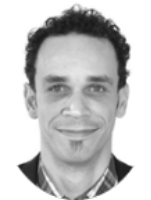
\includegraphics{david-folio.png}]{David Folio}
Use \texttt{IEEEbiography} with figure as option and the author name as
the argument followed by the biography text.
\end{IEEEbiography}
\begin{IEEEbiographynophoto}{John Doe}
Use \texttt{IEEEbiographynophoto} and the author name as the argument
followed by the biography text.
\end{IEEEbiographynophoto}
% that's all folks
\end{document}

